\section{Modelación}
\subsection{Modelación en SketchUp}
A partir de los planos de la figura \ref{fig: planos CAD} y de las mediciones más específicas de cada sala tomandas en terreno, se modeló las tres salas en el software SketchUp \cite{sketchup}, resultando los modelos de las Figuras \ref{fig: sketchup sala 1}, \ref{fig: sketchup sala 2} y \ref{fig: sketchup sala de ensayo}. Además, se tomó en consideración los muebles que utilizaban mayor volumen en las salas de reuniones. 
\begin{figure}[H]
    \centering
    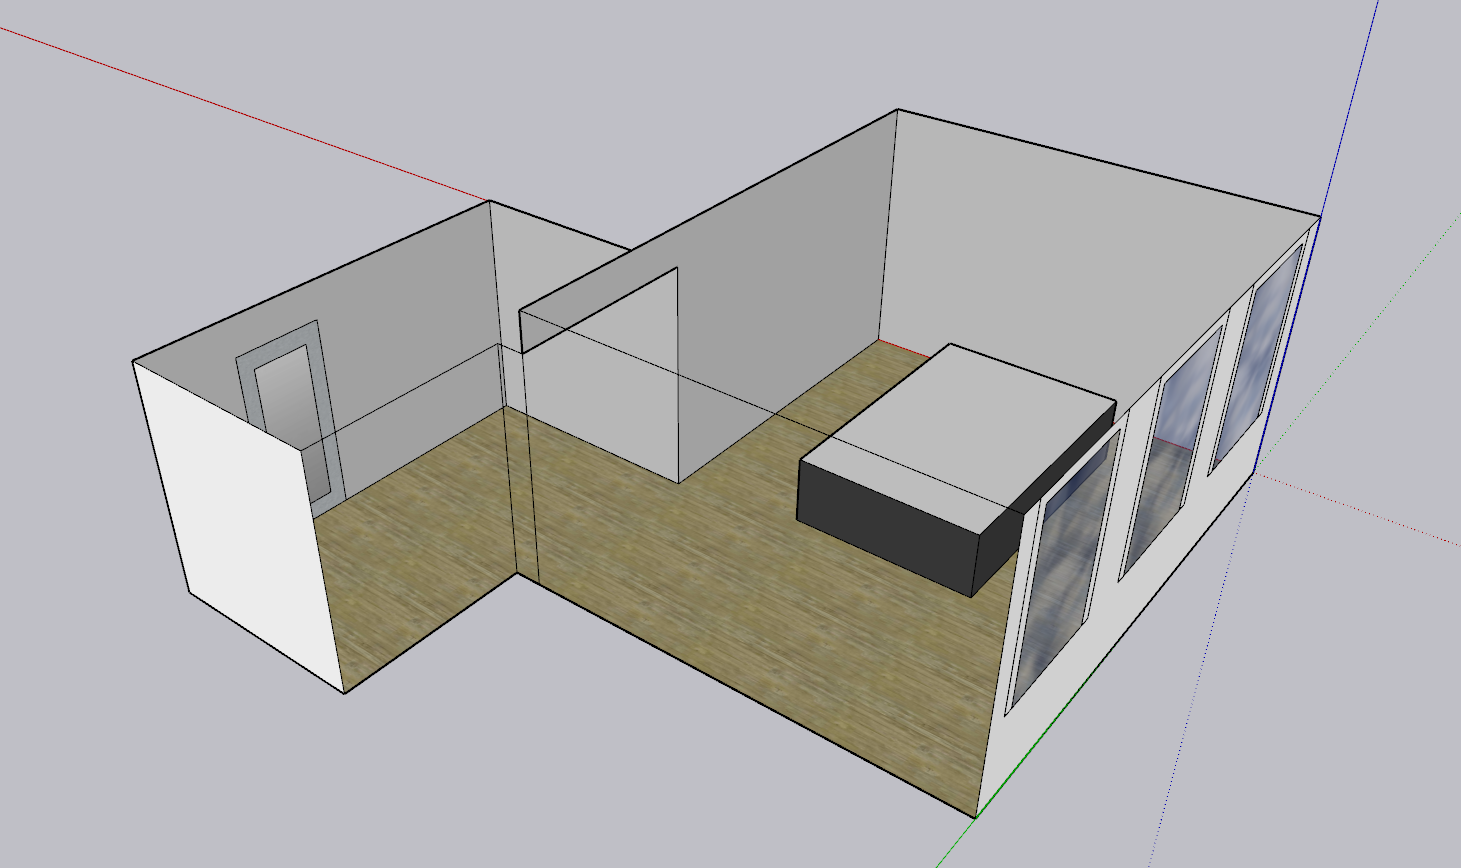
\includegraphics[width=8cm]{Imagenes/Modelacion/Sala 1 Sketchup.png}
    \caption{Modelo en SketchUp de Sala de reunión 1}
    \label{fig: sketchup sala 1}
\end{figure}

\begin{figure}[H]
    \centering
    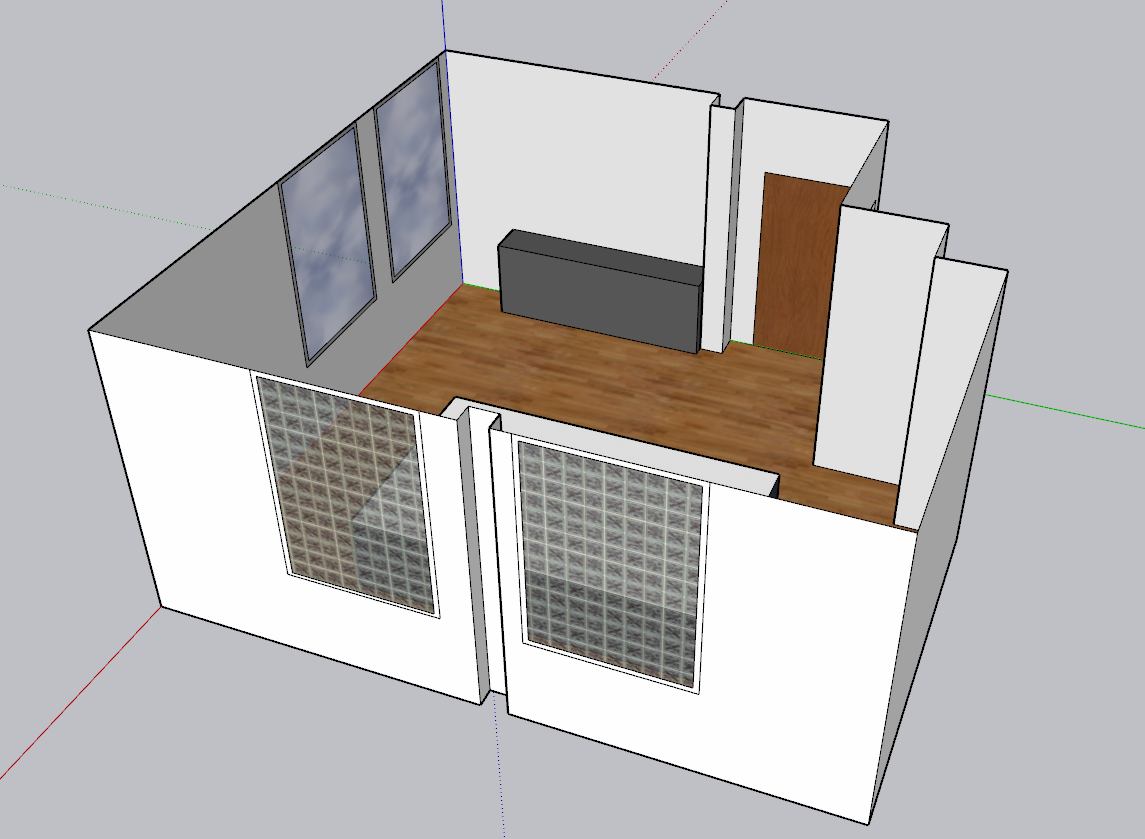
\includegraphics[width=8cm]{Imagenes/Modelacion/Sala 2 Sketchup.png}
    \caption{Modelo en SketchUp de Sala de reunión 2}
    \label{fig: sketchup sala 2}
\end{figure}

\begin{figure}[H]
    \centering
    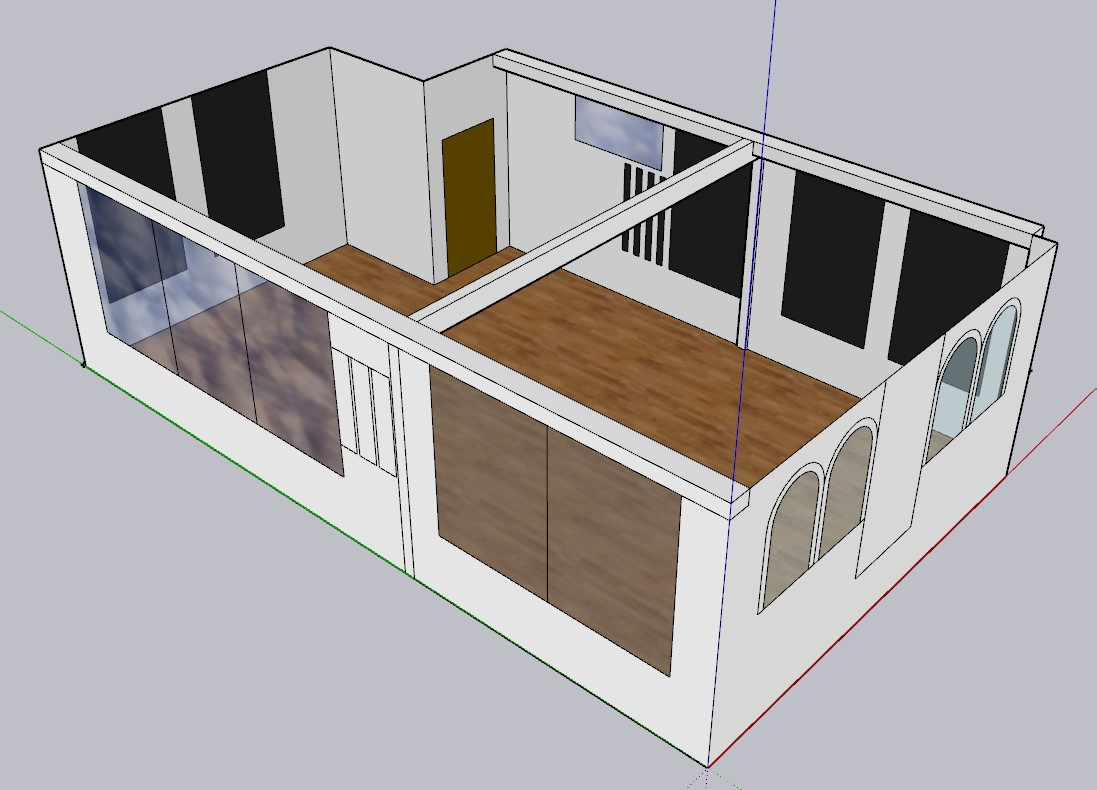
\includegraphics[width=8cm]{Imagenes/Modelacion/Sala ensayo Sketchup.jpg}
    \caption{Modelo en SketchUp de Sala de ensayo}
    \label{fig: sketchup sala de ensayo}
\end{figure}

\subsection{Modelación en EASE}
A partir de los modelos en SketchUp, estos se importaron al software EASE \cite{ease}, verificando las superficies y que estos estén bien cerrados para un correcto uso en en el programa. Para calibrar los modelos, se identificó los materiales de cada sala, para poder asignar los coeficientes de absorción a cada superficie correspondientemente. En la Tabla \ref{tab:materiales-ease} se pueden observar los materiales que se le asignaran a las distintas superficies y su respectivo coeficiente de absorción, además de la fuente de donde se extrajeron estos datos. Las superficies cuyo material es desconocido, fueron despejadas desde la ecuación \ref{eq:T60}.


\begin{table}[H]
    \centering
    \caption{Materiales utilizados para modelo en EASE.}
    \label{tab:materiales-ease}
    \begin{tabular}{|l|cccccc|c|}
    \hline
    \multirow{2}{*}{Material} & \multicolumn{6}{c|}{Frecuencia (Hz)}                                                                          & \multirow{2}{*}{Fuente} \\ \cline{2-7} 
            & \multicolumn{1}{c|}{$125$} & \multicolumn{1}{c|}{$250$} & \multicolumn{1}{c|}{$500$} & \multicolumn{1}{c|}{$1000$} & \multicolumn{1}{c|}{$2000$} & $4000$ & \\ \hline
    Parquet & \multicolumn{1}{c|}{$0.04$} & \multicolumn{1}{c|}{$0.04$} & \multicolumn{1}{c|}{$0.07$} & \multicolumn{1}{c|}{$0.06$} & \multicolumn{1}{c|}{$0.06$} &  $0.07$ & \cite{Recuero}\\ \hline
    Madera  & \multicolumn{1}{c|}{$0.25$} & \multicolumn{1}{c|}{$0.34$} & \multicolumn{1}{c|}{$0.18$} & \multicolumn{1}{c|}{$0.10$} & \multicolumn{1}{c|}{$0.10$} &  $0.06$ & \cite{Recuero}\\  \hline
    Black Acoustic Board (2") & \multicolumn{1}{c|}{$0.13$} & \multicolumn{1}{c|}{$0.75$} & \multicolumn{1}{c|}{$1.17$} & \multicolumn{1}{c|}{$1.14$} & \multicolumn{1}{c|}{$1.05$} & $1.09$ & \cite{blackboard}\\ \hline
    Vidrio  & \multicolumn{1}{c|}{$0.05$} & \multicolumn{1}{c|}{$0.5$} & \multicolumn{1}{c|}{$0.03$} & \multicolumn{1}{c|}{$0.03$} & \multicolumn{1}{c|}{$0.02$} & $0.02$ & \cite{Recuero}\\ \hline
    \end{tabular}
\end{table}

\noindent Para tener modelar la sala ocupada se consideró el siguiente coeficiente de absorción por persona,
que corresponde a una persona sentada en una silla:
\begin{table}[H]
    \centering
    \caption{Coeficiente de absorción de una persona sentada de EASE}
    \label{tab: coef abs persona}
    \begin{tabular}{|l|l|l|l|l|l|l|}
    \hline
    \textbf{Frecuencia Hz}      & $125$  & $250$  & $500$  & $1000$ & $2000$ & $4000$ \\ \hline
    \textbf{Absorción $\alpha$} & $0.31$ & $0.51$ & $0.73$ & $0.80$ & $0.82$ & $0.82$ \\ \hline
    \end{tabular}
\end{table}

\noindent Para simular a los músicos tocando en la sala de ensayo, se utilizó e ingresó al modelo de EASE distintos archivos GLL, provenientes
de una base de datos de mediciones de instrumentos grabados en una cámara anecóica con una arreglo esférico de micrófonos \cite{ackermann2023database}. 
De esta base de datos, se escogó los que componen la orquesta de cámara que ensaya en el lugar.

%insertar tabla con datos de cada instrumento
Estos instrumentos se ubicaron como se muestra en la Figura \ref{fig: EASE instrumentos}. Distribución que se estableció
a partir de imágenes recopiladas de la orquesta de cámara de Valdivia ensayando en el lugar (ver Figuras \ref{fig: ensayo cuerdas OCV} y \ref{fig: ensayo vientos OCV})
%ingresar imagen de distribución de instrumento en el EASE.
\begin{figure}
    \centering
    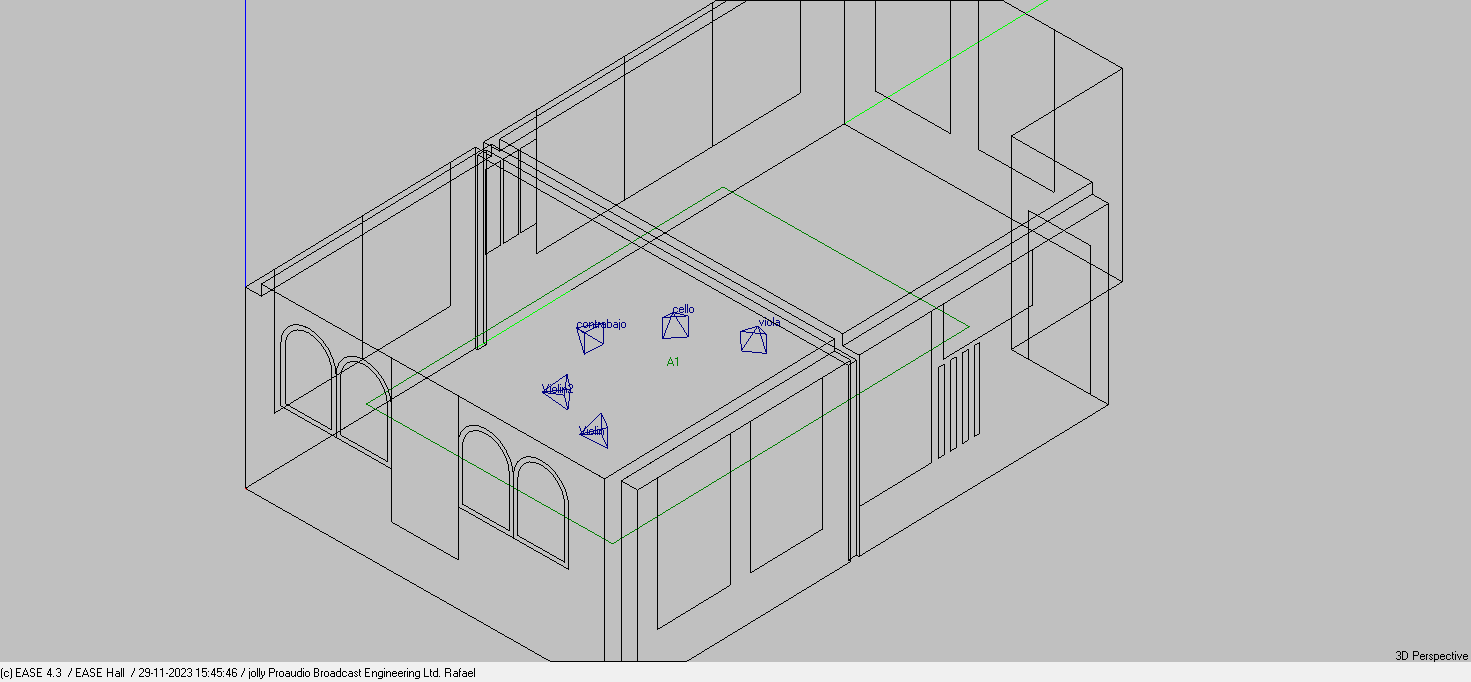
\includegraphics[width=11cm]{Imagenes/Modelacion/Instrumentos_ease.png}
    \caption{Imagen de la distribución de instrumentos en el EASE}
    \label{fig: EASE instrumentos}
\end{figure}
\begin{figure}[H]
    \centering
    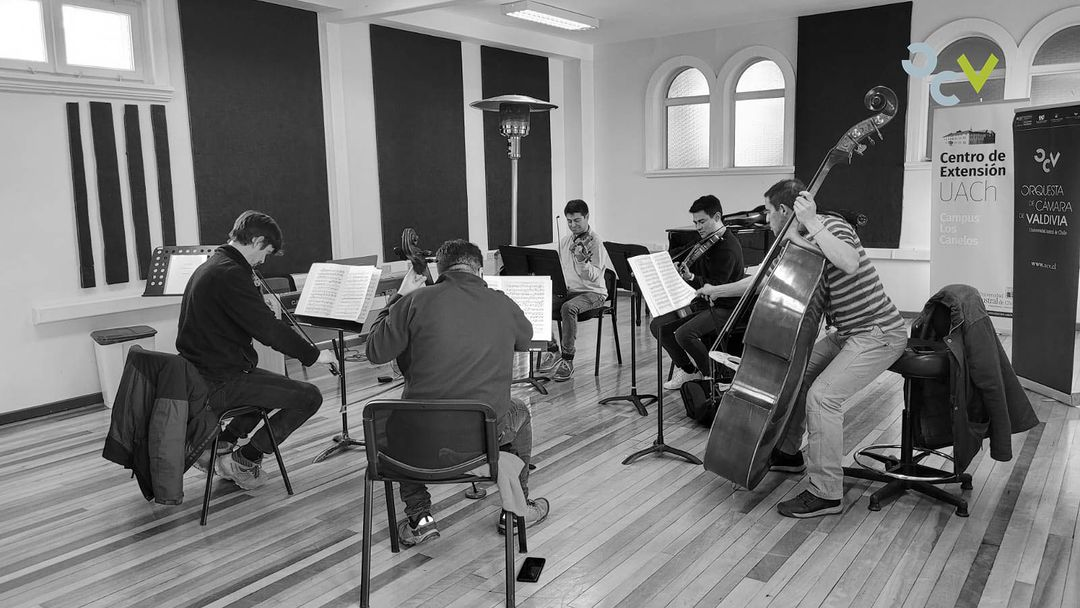
\includegraphics[width=11cm]{Imagenes/OCV/OCV cuerdas.jpg}
    \caption{Ensayo de cuerdas frotadas de orquesta de cámara en la sala de ensayo}
    \label{fig: ensayo cuerdas OCV}
\end{figure}

\begin{figure}[H]
    \centering
    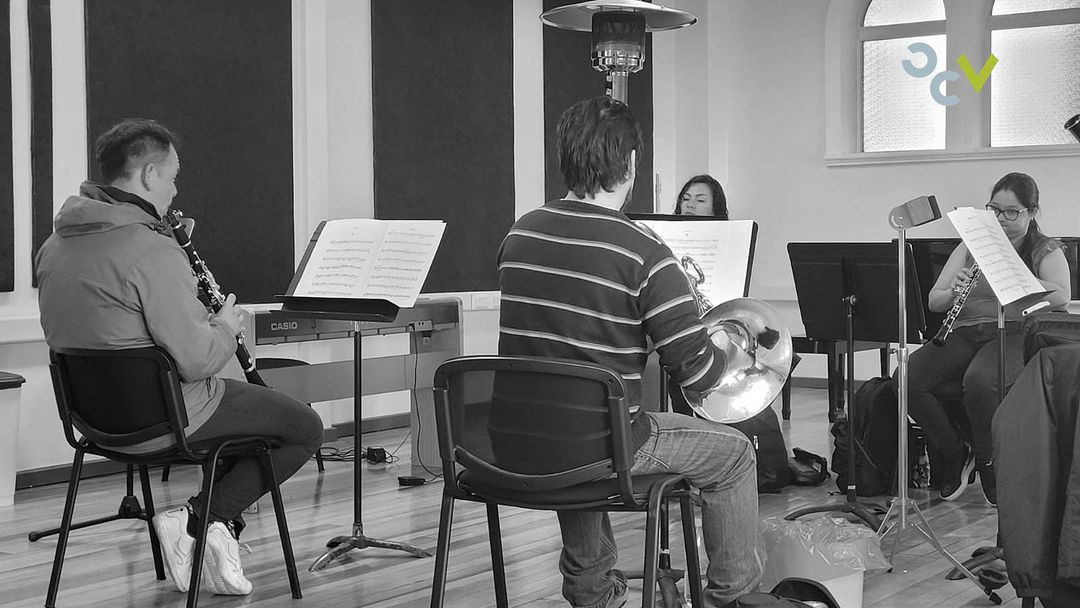
\includegraphics[width=11cm]{Imagenes/OCV/OCV vientos.jpg}
    \caption{Ensayo de bronces y maderas de la orquesta de cámara en la sala de ensayo}
    \label{fig: ensayo vientos OCV}
\end{figure}